% Curvatura como forma cuadrática: segunda forma fundamental, curvaturas principales, Euler y Meusnier
% Números y figuras PNG: apunte/scripts/cap13_curvatura.py (uv run python apunte/scripts/cap13_curvatura.py)
\chapter{Curvatura como forma cuadrática}\label{cap:curvatura}

\section{La idea}

Apoyá una regla sobre una naranja y después sobre una lata de gaseosa acostada en la mesa.
¿En qué se diferencian? Sobre la naranja, la regla toca la cáscara en un solo punto, en la
dirección que la pongas, y se separa de ella lo mismo hacia todos lados. Sobre la lata hay una
dirección, a lo largo, en la que la regla se apoya entera, y otra, alrededor, en la que se
separa enseguida. ¿Cuántos números hacen falta para decir cómo se curva una superficie en un
punto? La respuesta del capítulo: dos números y dos direcciones.

El capítulo~\ref{cap:cuatro-problemas} terminó comparando dos mediciones del mismo terreno
hechas en el plano; ahora dejamos el plano y medimos cuánto se curva una superficie. Imaginá
que apoyás una tabla rígida sobre una loma, de modo que toque el suelo en un solo punto: esa
tabla es el \emph{plano tangente}, el plano que mejor copia a la superficie en ese punto. Al
dar un paso en cualquier rumbo, el terreno se aparta de la tabla, y el apartamiento crece como
el cuadrado del paso: con un paso el doble de largo, el suelo queda cuatro veces más lejos de
la tabla. Medir la curvatura es medir ese
apartamiento rumbo por rumbo, y esa medida es una \emph{forma cuadrática} en el paso: una matriz simétrica de \(2\times2\) la contiene entera,
y sus autovalores y autovectores (capítulo~\ref{cap:autovectores}) dicen en qué rumbos la
superficie se curva más y menos.

\(r(u,v)\) es la regla que a cada par de números \((u,v)\), como el lugar de un
punto en una cuadrícula dibujada sobre la superficie, le asigna un punto del espacio, y
\(d=(du,dv)\) es un paso chico en esa cuadrícula. La primera forma \(I\) mide el largo del paso
sobre la superficie; la segunda, \(II\), cuánto se aparta la superficie del plano tangente al
darlo; \(E,F,G\) y \(L,M,N\) son las entradas de sus matrices. La normal \(n\) es la flecha de
largo uno perpendicular a la superficie, como un palito clavado derecho en el suelo. Las
curvaturas principales \(\kappa_1\) y \(\kappa_2\) (se lee \enquote{kappa}) son la mayor y la
menor curvatura entre todos los rumbos; \(K\), su producto, y \(H\), su promedio, las resumen en
un número. En el terreno, \(h(x,y)\) es la altura del suelo en el punto \((x,y)\) del mapa; una
\emph{loma} es una elevación redondeada, y una \emph{vaguada}, el fondo de un valle, por donde
corre el agua. Las curvaturas llevan signo respecto de la normal \(n\): con la normal hacia
arriba, una loma tiene curvaturas negativas y una vaguada, positivas.

\paragraph{En \(\R\): la segunda derivada.} Empecemos por una curva en el plano. Pensá en un
auto que recorre un camino de montaña: en una curva cerrada, el volante gira mucho por cada
metro recorrido; en una abierta, poco; en una recta, nada. Esa rapidez de giro es lo que
queremos medir. Si el gráfico de \(f\) tiene tangente horizontal
en \(0\), \(f(x)\approx f(0)+\tfrac12f''(0)\,x^2\): el apartamiento de la recta tangente es
la mitad de la segunda derivada por el cuadrado del paso. Llamamos \(\alpha\) al ángulo que
forma la tangente con una dirección fija y \(s\) a la distancia recorrida sobre la curva, la
\emph{longitud de arco}. La curvatura de una curva plana es
la rapidez con que gira su tangente por unidad de arco, \(\kappa=\lvert d\alpha/ds\rvert\): lo
que gira el volante por cada metro. Hay otra manera de verla. Imaginá que buscás, entre todas
las circunferencias tangentes a la curva en un punto, la que mejor se le pega. En cada punto
hay una circunferencia que mejor besa a la curva (la \emph{osculadora}) y
\(\kappa=1/\rho\), con \(\rho\) su radio: una curva cerrada se copia con una circunferencia
chica, y una abierta, con una grande. Para un gráfico,
\[
  \kappa=\frac{f''}{\bigl(1+f'^2\bigr)^{3/2}},
\]
con signo (positiva si la curva se dobla hacia arriba), y con tangente horizontal queda
\(\kappa=f''\): la segunda derivada \emph{es} la curvatura. La parábola \(y=x^2/2\) tiene en el
origen \(\kappa=1\) y su osculadora es la circunferencia de radio \(1\) centrada en \((0,1)\).

\paragraph{En \(\R^3\): una forma cuadrática.} Volvé a la regla apoyada sobre la lata: a lo
largo no se curva, alrededor sí, y en los rumbos intermedios, algo entre las dos cosas. Sobre una superficie, cada rumbo del plano
tangente tiene su propia curvatura. El apartamiento del plano tangente al dar el paso \(d\) es
\(\tfrac12\,II(d)=\tfrac12\bigl(L\,du^2+2M\,du\,dv+N\,dv^2\bigr)\) más términos de orden
superior, y la curvatura en el rumbo de \(d\) es el cociente \(II(d)/I(d)\) entre ese
apartamiento y el cuadrado del largo del paso. Como en el
capítulo~\ref{cap:svd}, una forma cuadrática se lee por sus ejes principales: hay dos rumbos
perpendiculares en los que la curvatura es máxima y mínima, y en los demás rumbos es un
promedio de esas dos con pesos \(\cos^2\theta\) y \(\sin^2\theta\) (Euler), donde \(\theta\) es
el ángulo que forma el rumbo con el de máxima curvatura.

\begin{idea}[La curvatura de una superficie es una forma cuadrática]
Dos números (los autovalores) y dos direcciones perpendiculares (los autovectores) dan la
curvatura en \emph{todos} los rumbos.
\end{idea}

\unidadInteractiva{12_curvatura}{Curvatura como forma cuadrática}{Explorá: elegí «silla z = (x² − y²)/4», llevá el punto a \((0,0)\) y girá el rumbo de \(0^\circ\) a \(90^\circ\). Mirá cómo \(\kappa_n\) pasa de \(0{,}5\) a \(-0{,}5\) y cómo, en \(45^\circ\), la sección normal deja de curvarse y el círculo osculador desaparece de la figura.}

{\small\vspace{1mm}\linkAnimacion{05_elipsoide_euler_meusnier}{Animación: Euler y Meusnier sobre el elipsoide}\par}

La animación muestra los dos teoremas del capítulo sobre el \emph{elipsoide}, la esfera apenas
achatada en los polos con que se describe la forma de la Tierra
(capítulo~\ref{cap:elipsoide}). Cortamos el elipsoide con un plano que contiene a la normal
y lo hacemos girar alrededor de ella: el radio osculador recorre los valores entre los dos
radios principales (Euler). Después inclinamos el plano hasta el del paralelo, la circunferencia
horizontal que pasa por el punto: el radio se achica con el coseno de la inclinación
(Meusnier).

\section{Construcciones, cuentas y ejemplos}

\subsection{Superficie, plano tangente y normal}

¿Cómo se describe una superficie con números? Imaginá una lámina de goma con una cuadrícula
dibujada, estirada sobre una loma. Cada punto de la lámina tiene dos números, su lugar en la
cuadrícula, y tres coordenadas en el espacio. Una superficie es la regla que pasa de los dos
números a las tres coordenadas, y es lo que necesitamos para hacer cuentas sobre el terreno, la
esfera o el elipsoide. Llamamos \(U\) a la región del plano donde viven los dos números, y
\(r_u\), \(r_v\) a las derivadas parciales de \(r\): las velocidades con que se mueve el punto
sobre la superficie cuando se avanza solo en \(u\) o solo en \(v\), que son las dos direcciones
de la cuadrícula estirada.

Sea \(r\colon U\subset\R^2\to\R^3\) una superficie con derivadas segundas continuas y
\(r_u\), \(r_v\) linealmente independientes. Las columnas de \(J=(r_u\ \ r_v)\) generan el plano
tangente; \(J\) es la matriz que convierte un paso en la cuadrícula en un paso en el espacio, y
la primera forma fundamental es la matriz \(J^TJ\) del
capítulo~\ref{cap:derivada} (sección~\ref{sec:metrica}):
\[
  I=\begin{pmatrix}E&F\\F&G\end{pmatrix}=J^TJ,\qquad I(d)=d^TI\,d=\lVert J\,d\rVert^2 ,
\]
el cuadrado del largo del vector tangente \(J\,d=r_u\,du+r_v\,dv\). Es la cinta métrica de la
superficie: \(E\) es el cuadrado del largo de un paso unitario en \(u\); \(G\), lo mismo en
\(v\); y \(F\) dice cuánto se apartan de ser perpendiculares las dos líneas de la cuadrícula
(si \(F=0\), se cruzan en ángulo recto). La normal unitaria es
\(n=r_u\times r_v/\lVert r_u\times r_v\rVert\), con \(n\cdot r_u=n\cdot r_v=0\): el palito
clavado derecho, perpendicular a las dos direcciones de la cuadrícula.
Cambiar el orden de los parámetros cambia \(n\) por \(-n\); todas las curvaturas con signo
cambian de signo con ella, y las que no dependen de esa elección son \(K\) y los valores
absolutos (\(K\), el producto de las dos curvaturas principales, se define en la
sección~\ref{sec:curvaturas-principales}).

\subsection{La segunda forma fundamental}\label{sec:segunda-forma}

Volvé a la tabla apoyada sobre la loma. Das un paso chico \(d\) en la cuadrícula: ¿cuánto
queda el suelo por debajo o por encima de la tabla? Del desplazamiento solo nos interesa la
parte que va según la normal; la que corre sobre la tabla no aparta nada. Las derivadas
primeras \(r_u\), \(r_v\) corren sobre la tabla, así que el apartamiento lo dan las derivadas
segundas, que dicen cómo cambian esas velocidades, y de ellas solo cuenta la componente según
\(n\). Para guardar esas tres componentes sirve la segunda forma fundamental.

\begin{definicion}[Segunda forma fundamental]\label{def:segunda-forma}
Los coeficientes de la segunda forma fundamental de \(r\) en un punto son las componentes
normales de las derivadas segundas,
\[
  L=r_{uu}\cdot n,\qquad M=r_{uv}\cdot n,\qquad N=r_{vv}\cdot n,
\]
y la segunda forma fundamental es la forma cuadrática
\[
  II(d)=L\,du^2+2M\,du\,dv+N\,dv^2
  =\begin{pmatrix}du&dv\end{pmatrix}\begin{pmatrix}L&M\\M&N\end{pmatrix}
  \begin{pmatrix}du\\dv\end{pmatrix}.
\]
\end{definicion}

Así, \(L\) dice cuánto se dobla la superficie hacia la normal al avanzar solo en \(u\); \(N\),
lo mismo al avanzar solo en \(v\); y \(M\) mezcla las dos direcciones. Estas \(M\) y \(N\) son
coeficientes; al final del capítulo las mismas letras vuelven como radios del elipsoide, y
allí se avisa. En la proposición que sigue, \(\operatorname{o}(\lVert d\rVert^2)\) (se lee
\enquote{o chica}) agrupa los términos que, divididos por \(\lVert d\rVert^2\), tienden a cero
cuando el paso se achica: lo que despreciamos.

\begin{proposicion}[II mide el apartamiento del plano tangente]\label{prop:II-taylor}
Para un paso \(d=(du,dv)\) en los parámetros, la distancia con signo de \(r(u+du,v+dv)\) al
plano tangente en \(r(u,v)\), medida según \(n\), es
\[
  \bigl(r(u+du,v+dv)-r(u,v)\bigr)\cdot n=\tfrac12\,II(d)+\operatorname{o}(\lVert d\rVert^2).
\]
\end{proposicion}

\begin{demostracion}
Por Taylor de segundo orden, componente a componente,
\[
  r(u+du,v+dv)-r(u,v)=r_u\,du+r_v\,dv
  +\tfrac12\bigl(r_{uu}\,du^2+2r_{uv}\,du\,dv+r_{vv}\,dv^2\bigr)+\operatorname{o}(\lVert d\rVert^2).
\]
Al multiplicar escalarmente por \(n\) los términos de primer orden se anulan, porque \(r_u\) y
\(r_v\) son tangentes, y los de segundo orden dan \(\tfrac12(L\,du^2+2M\,du\,dv+N\,dv^2)\).
\end{demostracion}

La primera forma mide el largo del paso; la segunda, cuánto se separa la superficie del plano
tangente al darlo: la curvatura sale de compararlas. En la imagen de la tabla, \(I\) es la cinta
con que medís cuánto caminaste, y \(\tfrac12II\), la regla vertical con que medís cuánto quedó
el suelo por encima o por debajo de la tabla.

\paragraph{Un terreno \(z=h(x,y)\).} El caso que más vamos a usar es el de un terreno
descripto por su altura: para cada punto \((x,y)\) del mapa, \(h(x,y)\) dice a qué altura está
el suelo. Las derivadas \(h_x\) y \(h_y\) dicen cuánto sube el terreno por metro hacia el eje
\(x\) y hacia el eje \(y\); las derivadas segundas \(h_{xx}\), \(h_{xy}\), \(h_{yy}\) dicen
cómo cambian esas inclinaciones, y son las entradas de la hessiana del
capítulo~\ref{cap:derivada}. Con \(r(x,y)=(x,\ y,\ h(x,y))\) queda
\(r_x=(1,0,h_x)\), \(r_y=(0,1,h_y)\), \(r_x\times r_y=(-h_x,-h_y,1)\) (la normal apunta hacia
arriba) y \(r_{xx}=(0,0,h_{xx})\), \(r_{xy}=(0,0,h_{xy})\), \(r_{yy}=(0,0,h_{yy})\). Con
\(W=\sqrt{1+h_x^2+h_y^2}\), un número que vale \(1\) en un terreno horizontal y crece con la
inclinación,
\[
  I=\begin{pmatrix}1+h_x^2&h_xh_y\\h_xh_y&1+h_y^2\end{pmatrix},\qquad
  II=\frac1W\begin{pmatrix}h_{xx}&h_{xy}\\h_{xy}&h_{yy}\end{pmatrix}.
\]
La matriz de \(II\) es la hessiana dividida por \(W\), y \(1/W\) es el coseno de la pendiente,
el ángulo que forma el terreno con la horizontal en la dirección en que más sube.

Pensá en la cima de un cerro o en el fondo de una cuenca: ahí la tabla queda horizontal y el
terreno no sube hacia ningún lado. En esos puntos, los puntos críticos de \(h\), todo se
simplifica.

\begin{proposicion}[En un punto crítico, II es la hessiana]\label{prop:II-hessiana}
Si \(\nabla h=0\) en el punto (plano tangente horizontal), entonces \(I\) es la identidad y
\(II\) es la hessiana de \(h\) (sección~\ref{sec:hessiana}).
\end{proposicion}

\begin{demostracion}
Con \(h_x=h_y=0\) resulta \(W=1\), \(E=G=1\) y \(F=0\).
\end{demostracion}

Fuera de un punto crítico las dos matrices difieren: la regla \(I\) deja de ser la identidad,
porque un paso horizontal \((dx,dy)\) se convierte en un paso más largo sobre la ladera, y
\(II\) se achica por el factor \(1/W\). En la imagen de la tabla: en una ladera la tabla queda
inclinada, y medir el apartamiento en vertical ya no es lo mismo que medirlo perpendicular a la
tabla.

\subsection{La curvatura normal}

Imaginá que caminás sobre la superficie siguiendo un camino cualquiera, siempre pegado al
suelo, y pasás por un punto en cierto rumbo. El suelo te obliga a curvar la trayectoria hacia
arriba o hacia abajo. ¿Cuánto? La proposición que sigue dice que eso depende solo del rumbo en
que pasás, no del camino que traías. Para enunciarla llamamos \(\gamma(t)\) al camino, con
\(t\) el tiempo; \((u(t),v(t))\) es su lugar en la cuadrícula en cada instante, \(\gamma'\) su
velocidad y \(\gamma''\) su aceleración.

\begin{proposicion}[Componente normal de la aceleración]\label{prop:curva-sobre-superficie}
Sea \(\gamma(t)=r(u(t),v(t))\) una curva sobre la superficie y \(d=(u',v')\) su velocidad en
los parámetros. Entonces \(\gamma'=J\,d\), \(\lVert\gamma'\rVert^2=I(d)\) y
\[
  \gamma''\cdot n=II(d).
\]
\end{proposicion}

\begin{demostracion}
Por la regla de la cadena, \(\gamma'=r_u\,u'+r_v\,v'\), y derivando otra vez,
\[
  \gamma''=r_{uu}\,u'^2+2r_{uv}\,u'v'+r_{vv}\,v'^2+r_u\,u''+r_v\,v'' .
\]
Al multiplicar por \(n\) los dos últimos términos se anulan.
\end{demostracion}

Toda curva sobre la superficie que pasa por el punto con la misma tangente tiene la misma
componente normal de la aceleración: la superficie se la impone. Si la curva está recorrida
por longitud de arco, a velocidad uno, \(\lVert\gamma'\rVert=1\) y \(\gamma''=\kappa\,\nu\), con \(\kappa\) su
curvatura y \(\nu\) (se lee \enquote{nu}) su normal principal, la flecha de largo uno hacia la
que dobla la curva; la proposición dice entonces que
\(\kappa\,\nu\cdot n=II(d)/I(d)\).

Entre todas las curvas que pasan con un rumbo dado hay una que se destaca. Tomá un cuchillo,
apoyá el filo sobre la superficie en el rumbo que te interesa y cortá derecho, con la hoja en
un plano que contiene a la normal: el borde del corte es una curva plana que sigue a la
superficie en ese rumbo sin inclinarse hacia ningún costado. Su curvatura es la que le
asignamos al rumbo, y se llama curvatura normal.

\begin{definicion}[Curvatura normal y sección normal]\label{def:curvatura-normal}
La \emph{curvatura normal} en el rumbo del paso \(d\neq0\) es
\[
  \kappa_n(d)=\frac{II(d)}{I(d)}=\frac{L\,du^2+2M\,du\,dv+N\,dv^2}{E\,du^2+2F\,du\,dv+G\,dv^2}.
\]
La \emph{sección normal} en ese rumbo es la curva que se obtiene al cortar la superficie con
el plano que contiene a \(n\) y al vector tangente \(J\,d\).
\end{definicion}

La sección normal es el borde del corte derecho con el cuchillo. Es una curva plana cuya normal principal está en su plano y es
perpendicular a la tangente: es \(\pm n\). Por la proposición~\ref{prop:curva-sobre-superficie},
su curvatura con signo respecto de \(n\) es \(\kappa_n(d)\). El signo depende de la normal
elegida: \(\kappa_n\) es positiva cuando la sección dobla hacia el lado al que apunta \(n\) y
negativa cuando dobla hacia el otro lado. Si cambiamos \(n\) por \(-n\), \(\kappa_n\) cambia de
signo, pero el radio de curvatura de la sección, \(R_n=1/\lvert\kappa_n(d)\rvert\), es el mismo. Además
\(\kappa_n(t\,d)=\kappa_n(d)\) para todo \(t\neq0\): depende solo del rumbo, no del largo
del paso. A distancia \(s\) sobre el plano tangente la sección se aparta
\(\tfrac12\kappa_n\,s^2\) de él, igual que la parábola en \(\R\).

Veamos las dos situaciones, en el fondo y en la ladera, sobre un paraboloide, una superficie
con forma de cuenco alargado.

\begin{ejemplo}[Paraboloide \(z=x^2/2+y^2/8\)]\label{ej:curv-paraboloide}
\emph{En el origen.} El gradiente se anula y la hessiana es
\(\operatorname{diag}(1;\ 0{,}25)\). Por la proposición~\ref{prop:II-hessiana}, \(I\) es la
identidad e \(II=\operatorname{diag}(1;\ 0{,}25)\): en el rumbo del eje \(x\) la curvatura
normal es \(1\) (radio \(1\)) y en el del eje \(y\), \(0{,}25\) (radio \(4\)). Las dos secciones
son las parábolas \(z=x^2/2\) y \(z=y^2/8\) de la figura~\ref{fig:curv-secciones}.

\emph{En el punto \((1,2)\).} Ahí \(z=1\), \(h_x=1\), \(h_y=0{,}5\) y \(W=\sqrt{2{,}25}=1{,}5\);
la hessiana es la misma (\(h\) es cuadrática), pero
\[
  I=\begin{pmatrix}2&0{,}5\\0{,}5&1{,}25\end{pmatrix},\qquad
  II=\frac1{1{,}5}\begin{pmatrix}1&0\\0&0{,}25\end{pmatrix}
  =\begin{pmatrix}0{,}6667&0\\0&0{,}1667\end{pmatrix},\qquad \det I=2{,}25 .
\]
En el rumbo del eje \(x\), \(d=(1,0)\), la curvatura normal es
\(\kappa_n=L/E=0{,}6667/2=0{,}3333\), y en el del eje \(y\), \(N/G=0{,}1667/1{,}25=0{,}1333\):
lejos del fondo, la superficie se curva bastante menos que lo que dice la hessiana, porque el
paso horizontal se estira sobre la ladera y la normal está inclinada. Las curvaturas
principales de este punto se calculan en el ejemplo~\ref{ej:curv-paraboloide-principales}.
\end{ejemplo}

\begin{figure}[htbp]
\centering
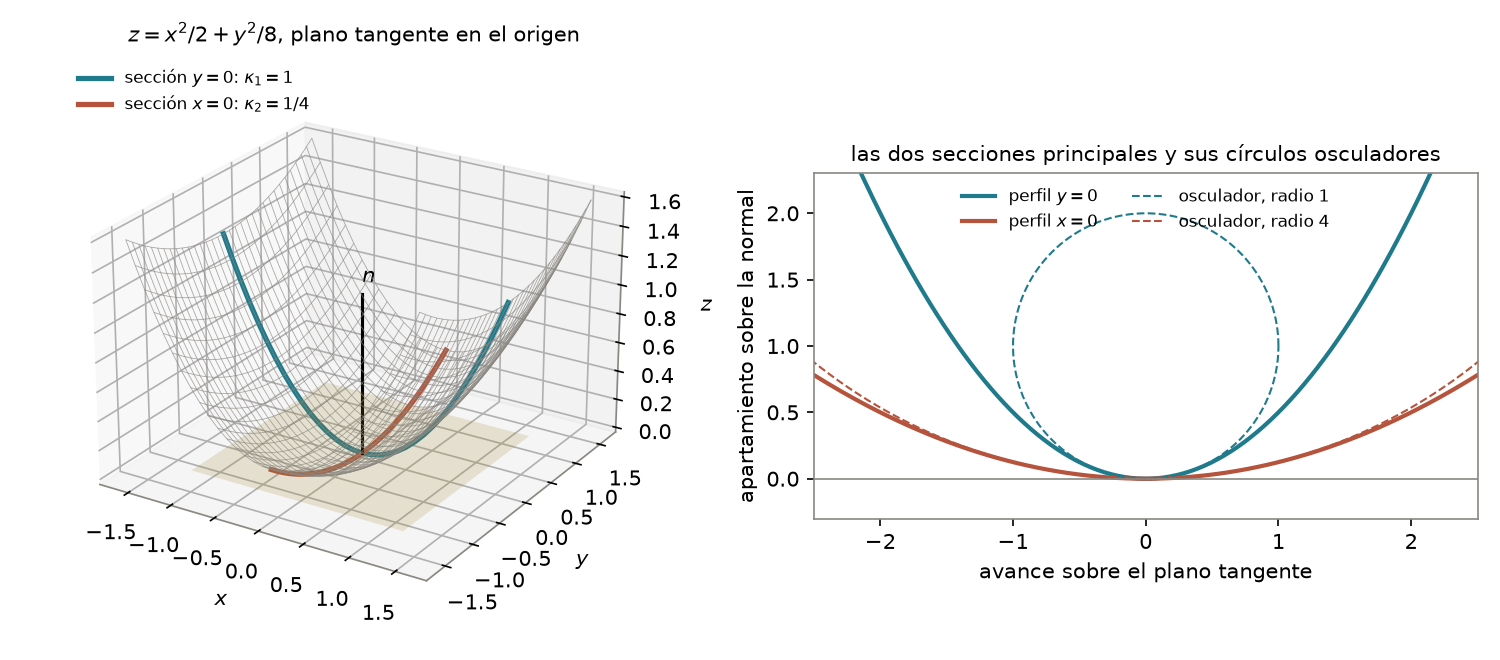
\includegraphics[width=\linewidth]{figuras/curvatura/curv_secciones.png}
\caption{Izquierda: el paraboloide \(z=x^2/2+y^2/8\) con su plano tangente en el origen (dorado),
la normal \(n\) y las dos secciones principales, sobre los ejes \(x\) (teal) e \(y\) (óxido).
Derecha: los dos perfiles con sus círculos osculadores, de radios \(1/\kappa_1=1\) y
\(1/\kappa_2=4\). Cerca del punto cada perfil se confunde con su círculo y el apartamiento del
plano tangente es \(\tfrac12\kappa_n s^2\).}
\label{fig:curv-secciones}
\end{figure}

\subsection{Curvaturas principales, direcciones principales y fórmula de Euler}\label{sec:curvaturas-principales}

Volvé al cuchillo y giralo alrededor de la normal, sin inclinarlo: el corte cambia de forma. En
la lata acostada, el corte a lo largo es una recta, el corte alrededor es una circunferencia, y
los intermedios son elipses, más curvadas cuanto más se acercan al corte alrededor. ¿En qué
rumbos se curva más y menos la superficie, y qué pasa en el medio? Saberlo sirve para leer la
forma de un terreno: en una loma alargada, el rumbo de mayor curvatura cruza la loma y el de
menor la sigue.

La curvatura normal es un cociente de dos formas cuadráticas. Si la cuadrícula de parámetros fuera
ortonormal (\(I\) la identidad), sus valores extremos serían los autovalores de \(II\). En
general no lo es, y la manera de reducirse a ese caso es medir el paso en una base ortonormal
del plano tangente, es decir, hacer un cambio de variables por congruencia
(sección~\ref{sec:congruencia}).

\begin{teorema}[Curvaturas principales y fórmula de Euler]\label{teo:euler}
En cada punto de la superficie:
\begin{enumerate}[label=(\alph*)]
  \item Los valores máximo y mínimo de \(\kappa_n\) entre todos los rumbos son las dos raíces
  \(\kappa_1\ge\kappa_2\) de
  \[
    \det(II-\kappa\,I)=0,
  \]
  que son los autovalores de \(S=I^{-1}II\). Se alcanzan en las direcciones \(d_1\), \(d_2\)
  que cumplen \((II-\kappa_iI)\,d_i=0\) (los autovectores de \(S\)), y si
  \(\kappa_1\neq\kappa_2\) esas direcciones son perpendiculares \emph{sobre la superficie}:
  \(d_1^TI\,d_2=0\).
  \item (Euler) Si \(\theta\) es el ángulo, medido sobre el plano tangente, entre un rumbo y
  la dirección \(d_1\), la curvatura normal en ese rumbo es
  \[
    \kappa_n(\theta)=\kappa_1\cos^2\theta+\kappa_2\sin^2\theta .
  \]
\end{enumerate}
\end{teorema}

En palabras: la matriz \(S\) junta las dos reglas, la que mide largos y la que mide
apartamientos, y sus autovalores son las curvaturas principales. Las direcciones \(d_1\) y
\(d_2\), donde la curvatura es máxima y mínima, se llaman \emph{direcciones principales}. Que
sean perpendiculares \enquote{sobre la superficie} quiere decir que se mide el ángulo con la
cinta \(I\), no en la cuadrícula: si la cuadrícula está estirada o torcida, dos direcciones
perpendiculares sobre el suelo pueden no parecerlo en el papel.

La demostración completa está en la sección~\ref{sec:curv-demostraciones}. La idea es esta: si
medimos el paso en una base ortonormal del plano tangente, la cinta \(I\) pasa a ser la
identidad y \(II\) queda como una matriz simétrica común; sus ejes principales
(sección~\ref{sec:simetricas}) son las direcciones principales, y escribir un rumbo cualquiera
como combinación de esos dos ejes da la fórmula de Euler. Con el cuchillo que gira: la curvatura
del corte pasa de \(\kappa_1\) a \(\kappa_2\) en un cuarto de vuelta, y cada rumbo intermedio es
un promedio de las dos.

Desarrollando el determinante, las curvaturas principales son las raíces de
\[
  (EG-F^2)\,\kappa^2-(EN-2FM+GL)\,\kappa+(LN-M^2)=0 ,
\]
y de los coeficientes salen su producto y su promedio.

¿Hay un número que diga, de un vistazo, si la superficie es como la naranja, como la lata o
como una silla de montar? El producto de las dos curvaturas lo dice por su signo; el promedio
dice cuánto se curva la superficie, en promedio, entre todos los rumbos.

\begin{definicion}[Curvatura de Gauss y curvatura media]\label{def:gauss-media}
\[
  K=\kappa_1\kappa_2=\frac{LN-M^2}{EG-F^2}=\frac{\det II}{\det I},\qquad
  H=\frac{\kappa_1+\kappa_2}2=\frac{EN-2FM+GL}{2(EG-F^2)}=\tfrac12\operatorname{tr}\bigl(I^{-1}II\bigr).
\]
\end{definicion}

\(K\) es la \emph{curvatura de Gauss} y \(H\), la \emph{curvatura media}; \(\operatorname{tr}\)
es la traza, la suma de la diagonal. Las unidades ayudan a leerlas: si las longitudes van en
metros, \(\kappa_1\), \(\kappa_2\) y \(H\) van en \(1/\mathrm{m}\) (la inversa de un radio) y
\(K\) en \(1/\mathrm{m}^2\).

\begin{idea}[Euler es la forma cuadrática en sus ejes principales]
Es la cuenta de la sección~\ref{sec:simetricas}; lo nuevo es que el ángulo \(\theta\) se mide
con la regla \(I\), sobre la superficie, y no en el plano de los parámetros.
\end{idea}

\paragraph{Consecuencias directas.} Como \(\cos^2(\theta+90^\circ)=\sin^2\theta\), dos rumbos
perpendiculares cualesquiera cumplen \(\kappa_n(\theta)+\kappa_n(\theta+90^\circ)=2H\), y el
promedio de \(\kappa_n\) sobre todos los rumbos es \(H\). ¿Hay superficies que se curvan igual
en todos los rumbos? La naranja del comienzo: la regla se separa de la cáscara lo mismo para
cualquier lado. Si \(\kappa_1=\kappa_2\), la
curvatura normal es la misma en todos los rumbos y el punto se llama \emph{umbilical}.

\paragraph{Clasificación de los puntos.} Pasá la mano por una silla de montar: a lo largo del
lomo del caballo la superficie sube hacia adelante y hacia atrás; de costado, baja hacia los
dos lados. En el terreno esa forma es un \emph{portezuelo}, el paso más bajo para cruzar una
sierra entre dos cerros. La naranja, la lata y la silla son los tres casos que importan, y el
signo de \(K\) los separa. El signo de \(K\) dice cómo se ubica la superficie
respecto de su plano tangente, igual que el criterio de la
proposición~\ref{prop:hessiana-criterio} para la hessiana:
\begin{itemize}
  \item \emph{Elíptico}, \(K>0\): las dos curvaturas tienen el mismo signo y, cerca del punto, la
  superficie queda de un solo lado del plano tangente (una cima, un fondo de cuenca).
  \item \emph{Hiperbólico}, \(K<0\): signos opuestos; la superficie cruza el plano tangente y hay
  dos rumbos \emph{asintóticos} en los que \(\kappa_n=0\), con
  \(\tan^2\theta=-\kappa_1/\kappa_2\) (un portezuelo).
  \item \emph{Parabólico}, \(K=0\) con una sola curvatura nula: en un rumbo la superficie se
  curva y en el perpendicular, no (un cilindro, el fondo de una canaleta).
  \item \emph{Plano}, \(\kappa_1=\kappa_2=0\): el segundo orden no alcanza para describir la forma.
\end{itemize}
En la silla de montar, los rumbos asintóticos son los dos rumbos intermedios en los que la mano
no sube ni baja: el corte derecho del cuchillo, en el punto, no se dobla hacia ningún lado.

Imaginá ahora que bajás la tabla del plano tangente, paralela a sí misma, una altura muy chica,
hasta que corta el suelo. ¿Qué forma tiene el corte? En una cima, una curva cerrada alrededor
del punto; en un portezuelo, dos pares de ramas que se abren.
La \emph{indicatriz de Dupin} lo resume en un dibujo: en las coordenadas \((y_1,y_2)\) sobre
\(e_1\), \(e_2\), las curvas \(\kappa_1y_1^2+\kappa_2y_2^2=\pm1\) son una elipse en un punto
elíptico, un par de hipérbolas con asíntotas en los rumbos asintóticos en uno hiperbólico, y
un par de rectas paralelas en uno parabólico. Acá \(e_1\) y \(e_2\) son las flechas de largo
uno, sobre el plano tangente, en las dos direcciones principales, y \((y_1,y_2)\) son las
coordenadas de un punto del plano tangente sobre esos dos ejes. En el rumbo \(\theta\), la distancia del centro a
la indicatriz es \(1/\sqrt{\lvert\kappa_n(\theta)\rvert}\). Como, por la
proposición~\ref{prop:II-taylor}, un plano paralelo al tangente y a altura \(\varepsilon\)
corta a la superficie, a menos de términos de orden superior, en la curva \(\tfrac12II=\varepsilon\), la indicatriz es la forma que
tienen las curvas de nivel muy cerca de un punto de tangente horizontal: elipses alrededor de
una cima, hipérbolas en un portezuelo (figura~\ref{fig:curv-euler}). Las \emph{curvas de nivel}
son las líneas de un mapa que unen los puntos de igual altura, y \(\varepsilon\) es la altura
chiquita a la que bajamos la tabla.

\begin{ejemplo}[Curvaturas principales del paraboloide en \((1,2)\)]\label{ej:curv-paraboloide-principales}
Con las matrices del ejemplo~\ref{ej:curv-paraboloide},
\[
  S=I^{-1}II=\frac1{27}\begin{pmatrix}10&-1\\-4&4\end{pmatrix}
  =\begin{pmatrix}0{,}3704&-0{,}0370\\-0{,}1481&0{,}1481\end{pmatrix}.
\]
Su traza es \(14/27\) y su determinante \(36/729=4/81\), así que \(H=7/27=0{,}2593\),
\(K=4/81=0{,}04938\) (que es \(\det II/\det I=0{,}1111/2{,}25\)), y
\[
  \kappa_{1,2}=\frac{7\pm\sqrt{13}}{27}:\qquad \kappa_1=0{,}3928,\quad \kappa_2=0{,}1257,
\]
con radios \(2{,}546\) y \(7{,}954\). La primera fila de \(S-\kappa I_2\) da las direcciones
\(d_1=(1,\ 3-\sqrt{13})\approx(1;\ -0{,}606)\) y \(d_2=(1,\ 3+\sqrt{13})\approx(1;\ 6{,}606)\).
En el plano de los parámetros no son perpendiculares (\(d_1\cdot d_2=1+(9-13)=-3\)), pero
sobre la superficie sí: \(d_1^TI\,d_2=2+0{,}5\cdot6+1{,}25\cdot(-4)=0\). Las tres
respuestas equivocadas que conviene descartar: los autovalores de la hessiana (\(1\) y
\(0{,}25\)), los de \(II\) sola (\(0{,}6667\) y \(0{,}1667\)) y las curvaturas en los ejes
(\(0{,}3333\) y \(0{,}1333\)). Las tres ignoran que la regla \(I\) no es la identidad. El
punto es elíptico, como todo el paraboloide.
\end{ejemplo}

\begin{ejemplo}[La silla \(z=(x^2-y^2)/4\)]\label{ej:curv-silla}
En el origen el gradiente se anula y \(II=\operatorname{diag}(0{,}5;\ -0{,}5)\), con \(I\) la
identidad: \(\kappa_1=0{,}5\) en el rumbo del eje \(x\), donde la superficie sube, y
\(\kappa_2=-0{,}5\) en el del eje \(y\), donde baja. \(K=-0{,}25\) (punto hiperbólico) y
\(H=0\). Por Euler,
\[
  \kappa_n(\theta)=0{,}5\cos^2\theta-0{,}5\sin^2\theta=0{,}5\cos2\theta ,
\]
que vale \(0{,}25\) en \(30^\circ\), \(0\) en \(45^\circ\) y \(-0{,}25\) en \(60^\circ\). Los
rumbos asintóticos cumplen \(\tan^2\theta=0{,}5/0{,}5=1\): son las diagonales, a \(45^\circ\)
de los ejes, y sobre ellas la superficie contiene a las rectas \(y=\pm x\), \(z=0\). La
figura~\ref{fig:curv-euler} muestra la curva de Euler y la indicatriz.
\end{ejemplo}

\begin{figure}[htbp]
\centering
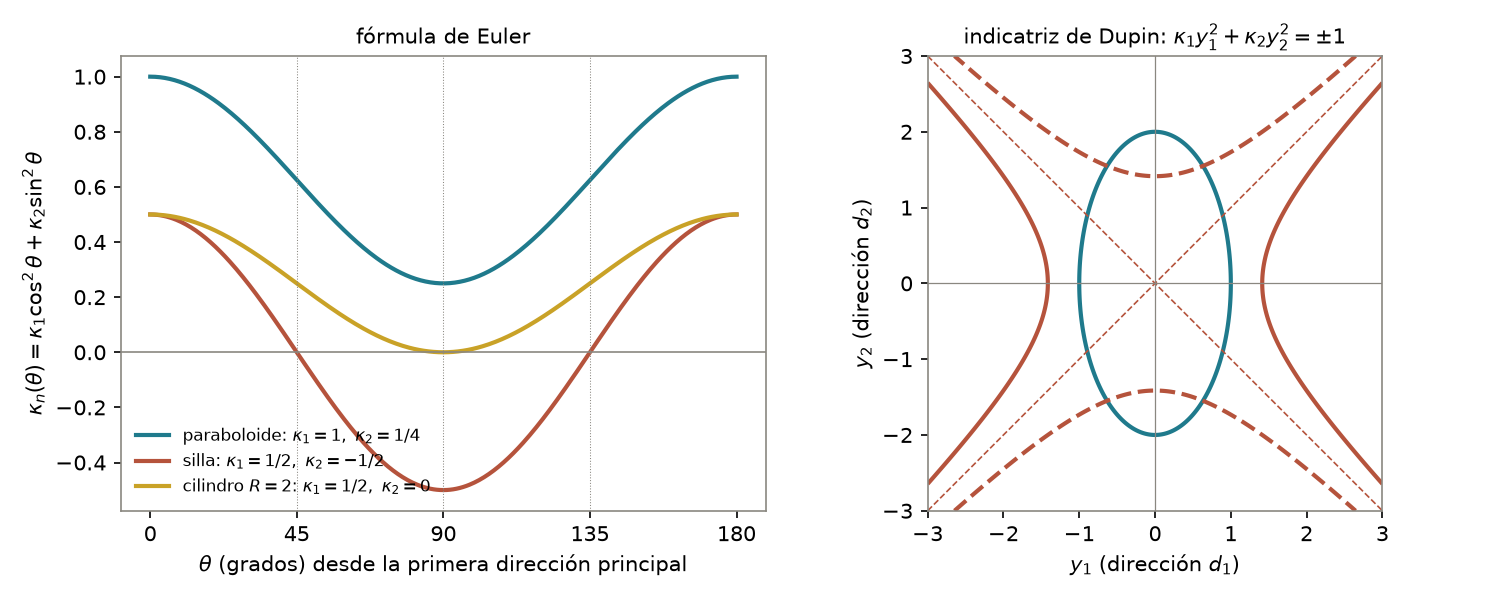
\includegraphics[width=\linewidth]{figuras/curvatura/curv_euler.png}
\caption{Izquierda: la fórmula de Euler \(\kappa_n(\theta)=\kappa_1\cos^2\theta+\kappa_2\sin^2\theta\)
para el paraboloide del ejemplo~\ref{ej:curv-paraboloide} en el origen (teal), la silla del
ejemplo~\ref{ej:curv-silla} (óxido) y un cilindro de radio \(2\) (dorado). Los extremos están
siempre a \(90^\circ\) uno de otro. Derecha: indicatriz de Dupin del paraboloide (elipse de
semiejes \(1/\sqrt{\kappa_1}=1\) y \(1/\sqrt{\kappa_2}=2\)) y de la silla (las hipérbolas
\(\kappa_1y_1^2+\kappa_2y_2^2=1\), llenas, y \(=-1\), de trazos), con sus asíntotas en los
rumbos asintóticos.}
\label{fig:curv-euler}
\end{figure}

Volvamos a la naranja y a la lata del comienzo, ahora con fórmulas: la esfera y el cilindro. En
la esfera usamos como parámetros la \emph{longitud} \(\lambda\), cuánto se gira alrededor del
eje desde un meridiano elegido (un \emph{meridiano} es un medio círculo que va de polo a polo), y
la \emph{latitud} \(\varphi\), cuánto se sube desde el ecuador; \(R\) es el radio. En el cilindro,
\(\vartheta\) (otra manera de escribir la letra theta) es el ángulo alrededor del eje, \(z\) la
altura, y las \emph{generatrices} son las rectas del cilindro paralelas a su eje: los rumbos en
los que la regla se apoyaba entera sobre la lata.

\begin{ejemplo}[Esfera y cilindro]\label{ej:curv-esfera-cilindro}
\emph{Esfera de radio \(R\).} Con longitud \(\lambda\) y latitud \(\varphi\), en ese orden,
\[
  r=R(\cos\varphi\cos\lambda,\ \cos\varphi\sin\lambda,\ \sin\varphi),
\]
y la normal \(r_\lambda\times r_\varphi\) normalizada es la exterior, \(n=r/R\). Derivando,
\[
  r_{\lambda\lambda}=-R(\cos\varphi\cos\lambda,\ \cos\varphi\sin\lambda,\ 0),\qquad
  r_{\varphi\varphi}=-r,\qquad
  r_{\lambda\varphi}=R(\sin\varphi\sin\lambda,\ -\sin\varphi\cos\lambda,\ 0),
\]
y la última es perpendicular a \(r\). Entonces
\[
  I=\begin{pmatrix}R^2\cos^2\varphi&0\\0&R^2\end{pmatrix},\qquad
  II=\begin{pmatrix}-R\cos^2\varphi&0\\0&-R\end{pmatrix}=-\frac1R\,I .
\]
Como \(II\) es múltiplo de \(I\), \(\kappa_n=-1/R\) en todos los rumbos: todos los puntos son
umbilicales, \(K=1/R^2\) y \(H=-1/R\) (con la normal interior, \(+1/R\)). El script del
capítulo lo verifica por diferencias finitas con \(R=2\) en \((\lambda,\varphi)=(0{,}3;\ 0{,}5)\):
\(I=\operatorname{diag}(3{,}0806;\ 4)\), \(II=\operatorname{diag}(-1{,}5403;\ -2)\) y
\(\kappa_1=\kappa_2=-0{,}5\). Para la Tierra como esfera de \(6371\) km,
\(1/R=0{,}000157\) 1/km.

\emph{Cilindro de radio \(R\).} Con parámetros \((\vartheta,z)\),
\[
  r=(R\cos\vartheta,\ R\sin\vartheta,\ z),\qquad n=(\cos\vartheta,\ \sin\vartheta,\ 0),\qquad
  r_{\vartheta\vartheta}=-(R\cos\vartheta,\ R\sin\vartheta,\ 0),
\]
la normal es la exterior y las otras derivadas segundas son nulas:
\[
  I=\begin{pmatrix}R^2&0\\0&1\end{pmatrix},\qquad II=\begin{pmatrix}-R&0\\0&0\end{pmatrix}.
\]
Las curvaturas principales son \(0\), en el rumbo de las generatrices, y \(-1/R\), en el de
las circunferencias: \(K=0\), todos los puntos son parabólicos, y en el rumbo a \(\theta\) de
la generatriz \(\kappa_n=-\sin^2\theta/R\).
\end{ejemplo}

Las dos cuentas confirman lo que se veía con la regla: en la naranja la curvatura es la misma
en todos los rumbos, y en la lata va de cero, a lo largo, a \(1/R\) en valor absoluto, alrededor.

\unidadInteractiva{12_curvatura}{Curvatura como forma cuadrática}{Verificá: con «cilindro: canaleta de radio 2.5 (eje y)» y el punto en \(x_0=0\), comprobá que \(\kappa_1=0{,}4=1/2{,}5\), \(\kappa_2=0\) y \(K=0\), y que con el rumbo en \(45^\circ\) la curvatura normal es \(0{,}2=0{,}4\cos^245^\circ\) (Euler). Después pasá a «esfera: cuenco de radio 2.5» y comprobá que \(\kappa_n\) no cambia al girar el rumbo y que \(K=0{,}16\).}

\subsection{El teorema de Meusnier: curvas oblicuas}

Volvé al cuchillo, pero ahora inclinalo: el filo sigue apoyado en el mismo rumbo, y la hoja ya
no contiene a la normal. ¿El corte se curva más o menos que el corte derecho? Probalo con la
naranja: un corte derecho por el centro deja una circunferencia grande, y uno inclinado, con el
mismo rumbo, una más chica. Cuanto más se inclina la hoja, más cerrada es la curva. Esto
permite calcular, por ejemplo, el radio de un paralelo de la Tierra a partir del radio de una
sección normal.

Una curva cualquiera sobre la superficie, por ejemplo un paralelo de la esfera, pasa por el
punto con un rumbo dado, pero su plano osculador no tiene por qué contener a la normal; su
curvatura queda determinada por la del rumbo y por la inclinación de su plano. El \emph{plano
osculador} de una curva es el plano en el que la curva dobla en ese punto, el que contiene a su
tangente y a su normal principal; para el corte inclinado del cuchillo, es el plano de la hoja.
En el teorema, \(p\) es el punto y \(\varphi\) mide la inclinación de la hoja respecto de la
normal (en el paralelo de la esfera esa inclinación coincide con la latitud, y por eso se usa
la misma letra).

\begin{teorema}[Meusnier]\label{teo:meusnier}
Sea \(\gamma\) una curva sobre la superficie que pasa por \(p\) con vector tangente en el
rumbo \(d\), con curvatura \(\kappa\neq0\) y normal principal \(\nu\), y sea \(\varphi\) el
ángulo entre \(\nu\) y la normal \(n\) de la superficie. Entonces
\[
  \kappa\cos\varphi=\kappa_n(d).
\]
Todas las curvas sobre la superficie con la misma tangente en \(p\) tienen la misma
curvatura normal; si además su curvatura \(\kappa\) no se anula, su radio es
\(\rho=1/\kappa=\rho_n\cos\varphi\), con \(\rho_n=1/\kappa_n\) el radio de la sección normal.
\end{teorema}

\begin{demostracion}
Recorremos \(\gamma\) por longitud de arco, de modo que su velocidad en los parámetros
\(d=(u',v')\) cumple \(I(d)=1\) y \(\gamma''=\kappa\,\nu\). Por la
proposición~\ref{prop:curva-sobre-superficie},
\(\kappa\cos\varphi=\kappa\,\nu\cdot n=\gamma''\cdot n=II(d)=II(d)/I(d)=\kappa_n(d)\).
\end{demostracion}

Como \(\cos\varphi\le1\), el radio de la curva oblicua nunca supera al de la sección normal: es
la naranja cortada en diagonal.

\paragraph{Hecho geométrico.} Llamamos \(C_n\) al centro de la osculadora de la sección normal
y \(C\) al de la osculadora de la curva oblicua; en esta subsección la letra \(C\) nombra
centros, no la matriz de cambio de base. Si \(\kappa_n\neq0\), el centro de la circunferencia osculadora
de la sección normal es \(C_n=p+\rho_n\,n\). El de la curva oblicua es \(p+\rho\,\nu\), con
\(\rho=\rho_n\cos\varphi\): es la proyección ortogonal de \(C_n\) sobre el plano osculador de
la curva. Las osculadoras de todas las curvas con esa tangente están sobre la esfera de radio
\(\rho_n\) centrada en \(C_n\), tangente a la superficie en \(p\); cada plano que contiene a
la tangente corta a esa esfera en una circunferencia, la osculadora de la curva
correspondiente (figura~\ref{fig:curv-meusnier}). Con el cuchillo: cualquiera sea la
inclinación de la hoja, la circunferencia que copia el corte está sobre esa misma esfera.

\begin{figure}[htbp]
\centering
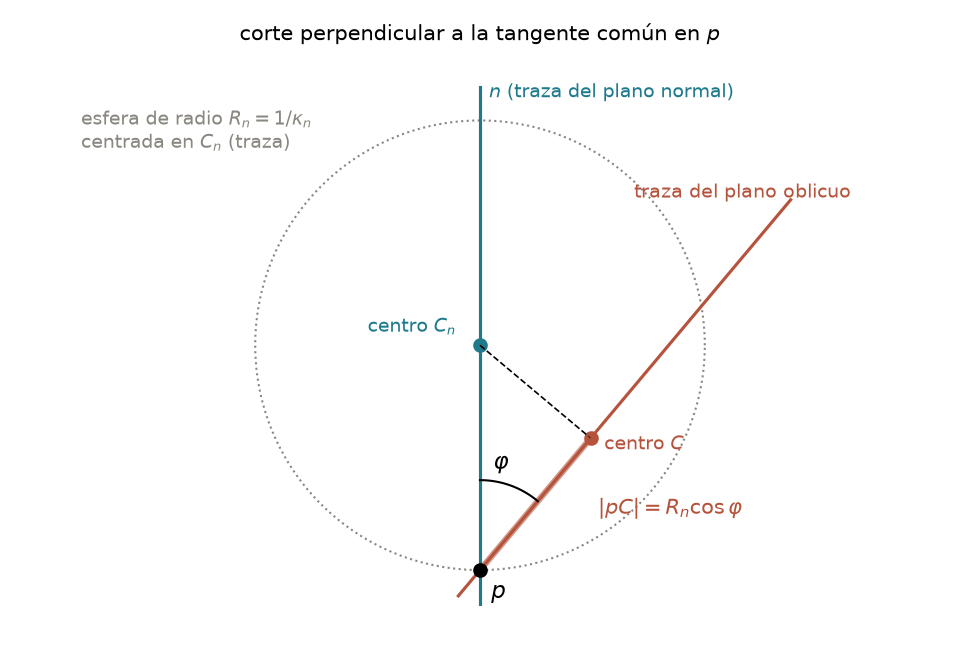
\includegraphics[width=.72\linewidth]{figuras/curvatura/curv_meusnier.png}
\caption{Teorema de Meusnier visto en el plano perpendicular a la tangente común. El plano
normal (teal) y un plano oblicuo (óxido), inclinado \(\varphi\) respecto de la normal,
contienen a la misma tangente. El centro \(C\) de la osculadora de la curva oblicua es la
proyección del centro \(C_n\) de la osculadora de la sección normal, y su radio es
\(\rho_n\cos\varphi\).}
\label{fig:curv-meusnier}
\end{figure}

El ejemplo que sigue termina en el elipsoide. Ahí los dos cortes normales que importan son el
del meridiano, que va de norte a sur, y el \emph{primer vertical}, el corte normal que va de
este a oeste, perpendicular al meridiano; \(N\) es el radio de curvatura del primer vertical, y
no el coeficiente de \(II\) que lleva la misma letra.

\begin{ejemplo}[Meusnier en el paraboloide y en el paralelo]\label{ej:curv-meusnier}
\emph{Paraboloide.} En el origen de \(z=x^2/2+y^2/8\), el rumbo del eje \(x\) tiene
\(\kappa_n=1\). Cortamos con el plano que contiene al eje \(x\) y está inclinado
\(\varphi=40^\circ\) respecto de la vertical: sus puntos son \(s\,(1,0,0)+q\,(0,\sin\varphi,\cos\varphi)\),
y la curva de corte cumple \(q\cos\varphi=s^2/2+(q\sin\varphi)^2/8\). Resolviendo \(q(s)\)
y derivando dos veces numéricamente en \(s=0\), la curvatura de esa curva plana resulta
\(1{,}30541\), y \(\kappa_n/\cos40^\circ=1{,}30541\): su radio es \(0{,}76604=1\cdot\cos40^\circ\).

\emph{Paralelo de la esfera.} El paralelo de latitud \(\varphi\) es una circunferencia de
radio \(R\cos\varphi\), y su normal principal apunta al eje, horizontal, formando el ángulo
\(\varphi\) con la normal interior de la esfera. Meusnier da
\(\kappa\cos\varphi=1/R\), o sea \(\kappa=1/(R\cos\varphi)\): el radio del paralelo es la
proyección del radio de la sección normal. En el elipsoide, la misma cuenta con la sección
normal perpendicular al meridiano (el primer vertical) da el radio del paralelo como
\(N\cos\varphi\), con \(N\) el radio del primer vertical
(sección~\ref{sec:radios-MN}).
\end{ejemplo}

\section{En profundidad}

\subsection{Demostración de las curvaturas principales y de la fórmula de Euler}\label{sec:curv-demostraciones}

Demostramos el teorema~\ref{teo:euler}. La estrategia es la del cuchillo que gira alrededor de
la normal: describimos los rumbos con una base ortonormal del plano tangente, donde medir
ángulos y largos es lo de siempre, y ahí la curvatura queda como una forma cuadrática común.
En la demostración, \(q_1,q_2\) son dos flechas de largo uno, perpendiculares, sobre el plano
tangente; \(Q\) es la matriz que las tiene por columnas; \(C\) es la matriz de cambio de base
que escribe las columnas de \(J\) en esa base (acá \(C\) vuelve a ser una matriz, no un
centro); y \(A\) es la matriz de \(II\) leída en la base nueva.

\begin{demostracion}
Sea \(q_1,q_2\) una base ortonormal del plano tangente y \(C\) la matriz de \(2\times2\) que
escribe las columnas de \(J\) en esa base: \(J=Q\,C\) con \(Q=(q_1\ \ q_2)\), \(Q^TQ=I_2\) (la
identidad de \(2\times2\)). Para un paso \(d\), el vector \(w=C\,d\) da las coordenadas
cartesianas del vector tangente \(J\,d=Q\,w\), y
\[
  I(d)=d^TJ^TJ\,d=d^TC^TC\,d=w^Tw .
\]
\(C\) es invertible porque \(r_u\), \(r_v\) son independientes. Con \(d=C^{-1}w\),
\[
  II(d)=w^T\,A\,w,\qquad A=C^{-T}\,II\,C^{-1},
\]
y \(A\) es simétrica, congruente con la matriz de \(II\). Por la
proposición~\ref{prop:simetrica} y la sección~\ref{sec:simetricas}, \(A\) tiene autovalores
reales \(\kappa_1\ge\kappa_2\) y autovectores unitarios perpendiculares \(e_1\), \(e_2\). Todo
rumbo unitario en el plano tangente se escribe \(w=\cos\theta\,e_1+\sin\theta\,e_2\), con
\(\theta\) el ángulo entre \(w\) y \(e_1\), y entonces
\[
  \kappa_n=\frac{w^TAw}{w^Tw}=\kappa_1\cos^2\theta+\kappa_2\sin^2\theta ,
\]
que es (b). Como es un promedio ponderado de \(\kappa_1\) y \(\kappa_2\), está entre los dos y
vale \(\kappa_1\) en \(\theta=0\) y \(\kappa_2\) en \(\theta=90^\circ\): son el máximo y el
mínimo. Falta traducir a la matriz \(S\). Como \(I=C^TC\),
\[
  C^{-1}AC=C^{-1}C^{-T}\,II=(C^TC)^{-1}II=I^{-1}II=S,
\]
así que \(S\) y \(A\) son conjugadas y tienen los mismos autovalores; si \(Ae_i=\kappa_ie_i\),
entonces \(d_i=C^{-1}e_i\) cumple \(Sd_i=\kappa_id_i\), o sea \((II-\kappa_iI)d_i=0\), y
\(\det(II-\kappa I)=\det I\,\det(S-\kappa I_2)\) se anula en los mismos \(\kappa\). Por último,
\(d_1^TI\,d_2=(Cd_1)^T(Cd_2)=e_1\cdot e_2=0\).
\end{demostracion}

Lo que hizo la demostración fue cambiar la cuadrícula estirada por una cuadrícula de cuadrados
perfectos apoyada sobre la tabla del plano tangente. Ahí la curvatura es una forma cuadrática
común, y las direcciones principales son sus ejes, perpendiculares; al volver a la cuadrícula
original, la perpendicularidad sigue valiendo, pero medida con \(I\).

\subsection{Cambio de parámetros: II se transforma por congruencia}

Imaginá que dos personas describen la misma loma con cuadrículas distintas: una con líneas
norte--sur y este--oeste cada metro, y otra girada y con pasos de dos metros. Las curvaturas
que calculen tienen que coincidir, porque la loma es la misma. ¿Qué cambia entonces de una
descripción a la otra, y qué no?

La curvatura no puede depender de la parametrización elegida. Sea \((u,v)=\phi(s,t)\) un cambio de parámetros con jacobiano
\(C=\partial(u,v)/\partial(s,t)\) invertible, y \(\tilde r(s,t)=r(\phi(s,t))\).
Acá \(\phi\) es la regla que pasa de la cuadrícula nueva, con números \((s,t)\), a la vieja; la
tilde marca lo que se calcula con la cuadrícula nueva; y \(C\), la matriz de derivadas de
\(\phi\), hace localmente el papel de la matriz de cambio de base del
capítulo~\ref{cap:cambio-base}.

\begin{proposicion}[Las dos formas fundamentales cambian por congruencia]\label{prop:II-congruencia}
Si \(\det C>0\) (la normal no cambia),
\[
  \tilde I=C^T\,I\,C,\qquad \tilde{II}=C^T\,II\,C .
\]
Si \(\det C<0\), la normal se invierte y \(\tilde{II}=-C^T\,II\,C\).
\end{proposicion}

\begin{demostracion}
Por la regla de la cadena (proposición~\ref{prop:regla-cadena}),
\((\tilde r_s\ \ \tilde r_t)=J\,C\), de donde \(\tilde I=C^TJ^TJ\,C=C^TIC\). Derivando otra vez,
\(\tilde r_{ss}=r_{uu}u_s^2+2r_{uv}u_sv_s+r_{vv}v_s^2+r_uu_{ss}+r_vv_{ss}\), y los dos últimos
términos son tangentes. Al multiplicar por \(n\) queda
\(\tilde r_{ss}\cdot n=(u_s,v_s)\,II\,(u_s,v_s)^T\); lo mismo con \(\tilde r_{st}\) y
\(\tilde r_{tt}\). En forma matricial, \(\tilde{II}=C^T\,II\,C\). Como
\(\tilde r_s\times\tilde r_t=\det C\,(r_u\times r_v)\), la normal solo se invierte si
\(\det C<0\).
\end{demostracion}

Es la regla de las formas cuadráticas de la tabla~\ref{tab:regla-de-cada-objeto}: un paso
\(\tilde d\) en los parámetros nuevos es el paso \(d=C\,\tilde d\) en los viejos, y
\(\tilde{II}(\tilde d)=II(C\tilde d)\). En cambio,
\[
  \tilde I^{-1}\tilde{II}=C^{-1}I^{-1}C^{-T}C^T\,II\,C=C^{-1}\,(I^{-1}II)\,C
\]
cambia por conjugación (sección~\ref{sec:conjugacion}): \(S=I^{-1}II\) es una transformación
lineal del plano tangente, no una forma cuadrática. Por eso sus autovalores \(\kappa_1\),
\(\kappa_2\), su determinante \(K\) y su traza \(2H\) no dependen de la parametrización, y sus
autovectores se transforman como vectores, \(\tilde d_i=C^{-1}d_i\). Los coeficientes \(L,M,N\)
por separado sí dependen de la cuadrícula. Que los autovalores de \(II\) sola no sean invariantes
(cambian con la congruencia) es otra manera de ver por qué no son las curvaturas.

Volviendo a las dos personas con cuadrículas distintas: anotan números distintos para \(E,F,G\)
y \(L,M,N\), pero coinciden en \(\kappa_1\), \(\kappa_2\), \(K\), \(H\) y en las direcciones
principales sobre el suelo.

\subsection{Hacia el elipsoide: los radios \texorpdfstring{\(M\)}{M} y \texorpdfstring{\(N\)}{N}}

¿Cuánto se curva la Tierra en el lugar del terreno que vamos a estudiar, y cómo se compara esa
curvatura con la de una loma? Para responder, reemplazamos la Tierra por el elipsoide, que
estudiamos en el capítulo~\ref{cap:elipsoide}.

En el elipsoide de revolución las direcciones principales son el meridiano y el primer
vertical, y las curvaturas principales son \(1/M\) y \(1/N\), con \(M\) el radio de curvatura
del meridiano y \(N\) el del primer vertical. La deducción por simetría está en la
proposición~\ref{prop:elip-principales} del capítulo~\ref{cap:elipsoide}, que también calcula
los radios (sección~\ref{sec:radios-MN}). Las
letras coinciden con las de los coeficientes de \(II\), pero son otra cosa: en esta subsección
\(M\) y \(N\) son radios.

Usamos el elipsoide GRS80, uno con medidas acordadas internacionalmente para representar la
Tierra entera (sus números están en el capítulo~\ref{cap:elipsoide}).
En la latitud \(-32{,}2133^\circ\) del centro del recorte de la
aplicación que sigue (el signo menos indica el hemisferio sur), \(M=6\,353\,560{,}5\) m y \(N=6\,384\,212{,}3\) m: las curvaturas
principales son \(1/M=0{,}0001574\) 1/km y \(1/N=0{,}0001566\) 1/km, la curvatura de Gauss
\(K=1/(MN)\) corresponde a una esfera de radio \(\sqrt{MN}=6368{,}9\) km, y el paralelo, por
Meusnier, tiene radio \(N\cos\varphi=5401{,}5\) km. Esos mismos radios dan el paso de una
cuadrícula de un segundo de arco: \(M\cdot1''=30{,}80\) m en sentido norte--sur y
\(N\cos\varphi\cdot1''=26{,}19\) m en sentido este--oeste. Un segundo de arco es la 3600-ava
parte de un grado; un arco de ese ángulo mide el radio por el ángulo en radianes, y por eso el
paso este--oeste, sobre el paralelo, es más corto.

\subsection{Aplicación topográfica: la curvatura de un terreno medido desde satélite}

Imaginá que tenés que describir la forma de una zona de sierras que nunca pisaste: dónde están
los filos, las líneas de cumbres de las que el agua se reparte hacia los dos lados; dónde las
vaguadas, por donde el agua se junta y corre; dónde los portezuelos para cruzar de un valle a
otro. No hace falta ir: hay mediciones de la altura del suelo de todo el planeta hechas desde
satélite. Con ellas armamos, alrededor de cada punto, una superficie que copia el terreno, y le
calculamos las curvaturas de este capítulo. ¿Qué dicen \(\kappa_1\), \(\kappa_2\) y sus
direcciones sobre una loma o una vaguada reales, y cuánto podemos confiar en esos números?

\begin{idea}[Esto lo vas a usar en Topografía]
Un \emph{modelo digital de elevación} (DEM, por sus siglas en inglés) es una cuadrícula de
alturas del terreno medidas desde satélite, con un valor cada \(30\) m. La altura de un punto se
llama \emph{cota}. Para copiar el terreno alrededor de un punto se elige la superficie que pasa
más cerca de muchas alturas medidas, como en el capítulo~\ref{cap:inversas}.
\end{idea}

\paragraph{El dato.} Usamos el modelo de superficie Copernicus DEM GLO-30 (un segundo
de arco, unos \(30\) m), en un recorte de \(512\times512\) celdas de la precordillera de
Mendoza: latitudes entre \(-32{,}284^\circ\) y \(-32{,}142^\circ\), longitudes entre
\(-69{,}000^\circ\) y \(-68{,}858^\circ\), alturas entre \(1014\) y \(2989\) m. Es un modelo de
superficie: incluye lo que esté sobre el suelo, como árboles y construcciones.
Los centros de celda están en segundos enteros; el paso en metros sale de la subsección
anterior: \(26{,}2\) m hacia el este y \(30{,}80\) m hacia el norte. Ponemos un sistema local
con origen en la celda central de cada ventana, \(x\) hacia el este, \(y\) hacia el norte y
\(z\) la altura.

\paragraph{La cuadrática local.} Imaginá que apoyás sobre el terreno, alrededor de cada punto,
una lámina flexible que solo puede tomar forma de cuenco, de domo, de canaleta o de silla, y la
acomodás para que pase lo más cerca posible de las alturas medidas. Esa lámina es una
cuadrática, y sus curvaturas son las que buscamos. La \emph{ventana} es el cuadrado de celdas
que usamos para acomodarla. En una ventana de \(7\times7\) celdas
(\(157\times185\) m) alrededor de cada punto calculamos
\[
  z=a+b\,x+c\,y+d\,x^2+e\,xy+f\,y^2
\]
eligiendo los seis coeficientes que hacen más chica la suma de los cuadrados de las diferencias
con las alturas medidas: \(49\) ecuaciones y \(6\) incógnitas, resueltas con las ecuaciones
normales de la sección~\ref{sec:ecuaciones-normales}. Los coeficientes se leen así: \(a\) es la
altura del centro; \(b\) y \(c\), cuánto sube el terreno por metro hacia el este y hacia el
norte; \(d\), \(e\), \(f\), cómo se curva. (Esta \(d\) es un número, no el paso \(d\) del resto
del capítulo; tampoco \(e\) tiene que ver con los vectores \(e_1\), \(e_2\).) De ahí \(h_x=b\), \(h_y=c\) y la
hessiana \(\left(\begin{smallmatrix}2d&e\\e&2f\end{smallmatrix}\right)\) en el centro; con las
fórmulas del terreno de la sección~\ref{sec:segunda-forma} armamos \(I\) e \(II\), y las
curvaturas principales salen de \(I^{-1}II\) (teorema~\ref{teo:euler}). Las direcciones
principales se dan por su \emph{acimut}, el ángulo que forma la proyección horizontal
\((dx,dy)\) de cada dirección con el norte, medido desde el
norte en sentido horario: \(0^\circ\) es el norte, \(90^\circ\) el este, \(180^\circ\) el sur.

Elegimos tres puntos mirando el relieve (figura~\ref{fig:curv-dem}): una loma en el
extremo noreste del recorte, una vaguada en el sur y una silla en el norte. El
cuadro~\ref{tab:curv-dem} reúne los resultados. Además de las curvaturas, el cuadro da cuánto se
separan, en promedio cuadrático, las \(49\) alturas medidas de la lámina (entre \(5\) y \(7\) m);
la pendiente, en grados y en porcentaje (metros que se sube cada \(100\) m de avance
horizontal); y la dirección de la bajada, hacia donde el terreno desciende más rápido.

\begin{table}[htbp]
\centering
\small
\caption{Cuadrática local en ventanas de \(7\times7\) celdas del DEM Copernicus GLO-30.
Coeficientes \(d,e,f\) en \(10^{-3}\) 1/m; curvaturas en 1/km; radios en m; acimutes en
grados desde el norte. Las curvaturas llevan signo respecto de la normal hacia arriba.}
\label{tab:curv-dem}
\begin{tabular}{lccc}
 & loma & vaguada & silla\\\hline
fila, columna del recorte & \(48,\ 466\) & \(420,\ 252\) & \(31,\ 118\)\\
latitud, longitud & \(-32{,}1556^\circ,\ -68{,}8706^\circ\) & \(-32{,}2589^\circ,\ -68{,}9300^\circ\) & \(-32{,}1508^\circ,\ -68{,}9672^\circ\)\\
cota de la celda (m) & \(1785{,}4\) & \(1438{,}2\) & \(1924{,}7\)\\
\(b,\ c\) & \(0{,}0944;\ 0{,}2008\) & \(0{,}0084;\ 0{,}1087\) & \(0{,}0123;\ 0{,}0751\)\\
\(d,\ e,\ f\) & \(-6{,}806;\ 3{,}427;\ -1{,}688\) & \(6{,}862;\ -1{,}720;\ 0{,}200\) & \(3{,}232;\ -1{,}095;\ -3{,}033\)\\
residuo rms (m) & \(6{,}12\) & \(5{,}18\) & \(6{,}81\)\\
pendiente & \(12{,}5^\circ\) (22{,}2\,\%) & \(6{,}2^\circ\) (10{,}9\,\%) & \(4{,}4^\circ\) (7{,}6\,\%)\\
acimut de la bajada & \(205{,}2\) & \(184{,}4\) & \(189{,}3\)\\
autovalores de la hessiana & \(-2{,}335;\ -14{,}653\) & \(13{,}943;\ 0{,}181\) & \(6{,}559;\ -6{,}160\)\\
\(\kappa_1;\ \kappa_2\) & \(-2{,}174;\ -14{,}292\) & \(13{,}860;\ 0{,}178\) & \(6{,}539;\ -6{,}107\)\\
radios \(1/\lvert\kappa_1\rvert;\ 1/\lvert\kappa_2\rvert\) & \(460;\ 70\) & \(72;\ 5610\) & \(153;\ 164\)\\
acimut de \(d_1;\ d_2\) & \(17{,}0;\ 107{,}4\) & \(97{,}2;\ 7{,}2\) & \(95{,}0;\ 4{,}9\)\\
\(K\) (1/km\(^2\)); \(H\) (1/km) & \(31{,}08;\ -8{,}233\) & \(2{,}471;\ 7{,}019\) & \(-39{,}94;\ 0{,}216\)
\end{tabular}
\end{table}

\paragraph{La lectura.} En la \emph{loma} las dos curvaturas son negativas (punto elíptico,
convexo): la superficie cae hacia los dos lados. Cae fuerte en el rumbo de
\(107^\circ\), con radio de \(70\) m, que es el que cruza el filo, y apenas en el de
\(17^\circ\), con radio de \(460\) m, que es el que lo sigue: es un espolón, una loma alargada
que baja desde las cumbres, en este caso hacia el
sur-suroeste (la bajada apunta a \(205^\circ\), casi sobre \(d_1\)). En la
\emph{vaguada} hay una curvatura positiva fuerte, \(13{,}86\) 1/km (radio de \(72\) m), en el
rumbo \(97^\circ\), que cruza el cauce, y otra casi nula en el rumbo \(7^\circ\), a lo largo
del cauce: el punto es casi parabólico, con \(K\) chica, como una canaleta que baja hacia el
sur. En la \emph{silla} los signos son opuestos y casi iguales en valor absoluto
(\(K<0\), \(H\approx0\)): el terreno sube hacia el este y el oeste y baja hacia el norte y el
sur, la forma de un portezuelo. Con pendientes de \(4{,}4^\circ\) a \(12{,}5^\circ\) la corrección por
la pendiente es chica pero visible: los autovalores de la hessiana difieren de las curvaturas
principales hasta en un \(7{,}4\)\,\% en la loma, la de mayor pendiente, por el factor \(1/W\) y por la
regla \(I\). Las direcciones principales son perpendiculares sobre la superficie
(\(d_1^TI\,d_2=0\)); sus proyecciones horizontales lo son casi (en la loma, \(107{,}4-17{,}0=90{,}4^\circ\)).
Son los tres casos de la naranja, la lata y la silla de montar, ahora en un cerro de verdad: la
loma es un domo alargado, la vaguada una canaleta, como media lata con el hueco hacia arriba, y el portezuelo la
silla.

\paragraph{Verificación con Euler a lo largo de la máxima pendiente.} ¿Cómo sabemos que las
cuentas están bien? Calculamos lo mismo por caminos distintos y comparamos. La \emph{línea de
máxima pendiente} es la que sigue, desde el punto, la dirección en que el terreno baja más
rápido. El plano vertical que
contiene a la línea de máxima pendiente contiene también a la normal, porque
\(n\propto(-h_x,-h_y,1)\) está en él: el perfil del terreno según la máxima pendiente
\emph{es} una sección normal. Su curvatura se puede calcular de tres maneras
independientes: con Euler, a partir de \(\kappa_1\), \(\kappa_2\) y del ángulo \(\theta\) que
forma ese rumbo con \(d_1\) sobre la superficie; directamente como \(II(d)/I(d)\); y como la
curvatura \(h''/(1+h'^2)^{3/2}\) de la curva plana que es el perfil de la cuadrática. Las tres
coinciden en los tres puntos:
\begin{center}
\begin{tabular}{lccc}
 & loma & vaguada & silla\\\hline
\(\theta\) entre la máxima pendiente y \(d_1\) & \(8{,}0^\circ\) & \(87{,}2^\circ\) & \(85{,}7^\circ\)\\
Euler, \(II/I\) y perfil de la cuadrática (1/km) & \(-2{,}410\) & \(0{,}211\) & \(-6{,}035\)\\
perfil del DEM interpolado (1/km) & \(-4{,}064\) & \(1{,}259\) & \(-7{,}883\)
\end{tabular}
\end{center}
La última fila es un control con el dato crudo: interpolamos las alturas medidas (bilineal: un
promedio ponderado de las cuatro celdas vecinas) a lo largo de
la línea de máxima pendiente, \(\pm3\) celdas, y buscamos la parábola que mejor lo copia. Tiene el mismo
signo y el mismo orden de magnitud, con diferencias de \(1\) a \(2\) 1/km: el perfil usa solo
los datos de una línea, mientras que la cuadrática promedia la ventana entera. Diferencias de
ese tamaño son la resolución real de una curvatura calculada con alturas cada \(30\) m, como
muestra el cambio de ventana: con ventanas de \(5\times5\), \(7\times7\) y \(9\times9\)
celdas, \(\kappa_2\) de la loma da \(-19{,}75\), \(-14{,}29\) y \(-11{,}01\) 1/km, y
\(\kappa_1\) de la vaguada, \(20{,}44\), \(13{,}86\) y \(10{,}19\) 1/km. La curvatura de un
terreno depende de la escala a la que se mira, y la ventana es parte del resultado.

\paragraph{Meusnier a lo largo de la curva de nivel.} En el rumbo de la curva de nivel (en la
loma, \(115{,}2^\circ\) desde el norte) la tangente es horizontal y la sección \emph{vertical} no es
normal: su normal principal es vertical y forma con \(n\) el ángulo de la pendiente, con
\(\cos\varphi=1/W=0{,}9762\). Es el cuchillo inclinado de la subsección de Meusnier: cortamos en
vertical, pero la normal del terreno está inclinada. Su curvatura es la segunda derivada del perfil,
\(-14{,}398\) 1/km, y por Meusnier \(-14{,}398\cdot0{,}9762=-14{,}056\) 1/km, que coincide con
\(\kappa_n=II(d)/I(d)=-14{,}056\) 1/km en ese rumbo.

\paragraph{Escala y mapa.} El \(\kappa_1\) de la vaguada es \(88\,274\) veces la curvatura
de la Tierra, \(1/\sqrt{MN}\): para estudiar la forma del terreno a esta escala el plano de
referencia alcanza. Repitiendo la cuenta en cada celda se obtiene un mapa de curvatura media
(figura~\ref{fig:curv-dem}): las vaguadas aparecen como líneas azules (\(H>0\)), los filos como
líneas rojas (\(H<0\)). En el recorte, el \(38{,}8\)\,\% de las celdas tiene \(K>0\) y el
\(61{,}2\)\,\% tiene \(K<0\); el \(90\)\,\% de los valores de \(H\) está entre \(-2{,}38\) y
\(2{,}13\) 1/km.

\begin{figure}[htbp]
\centering
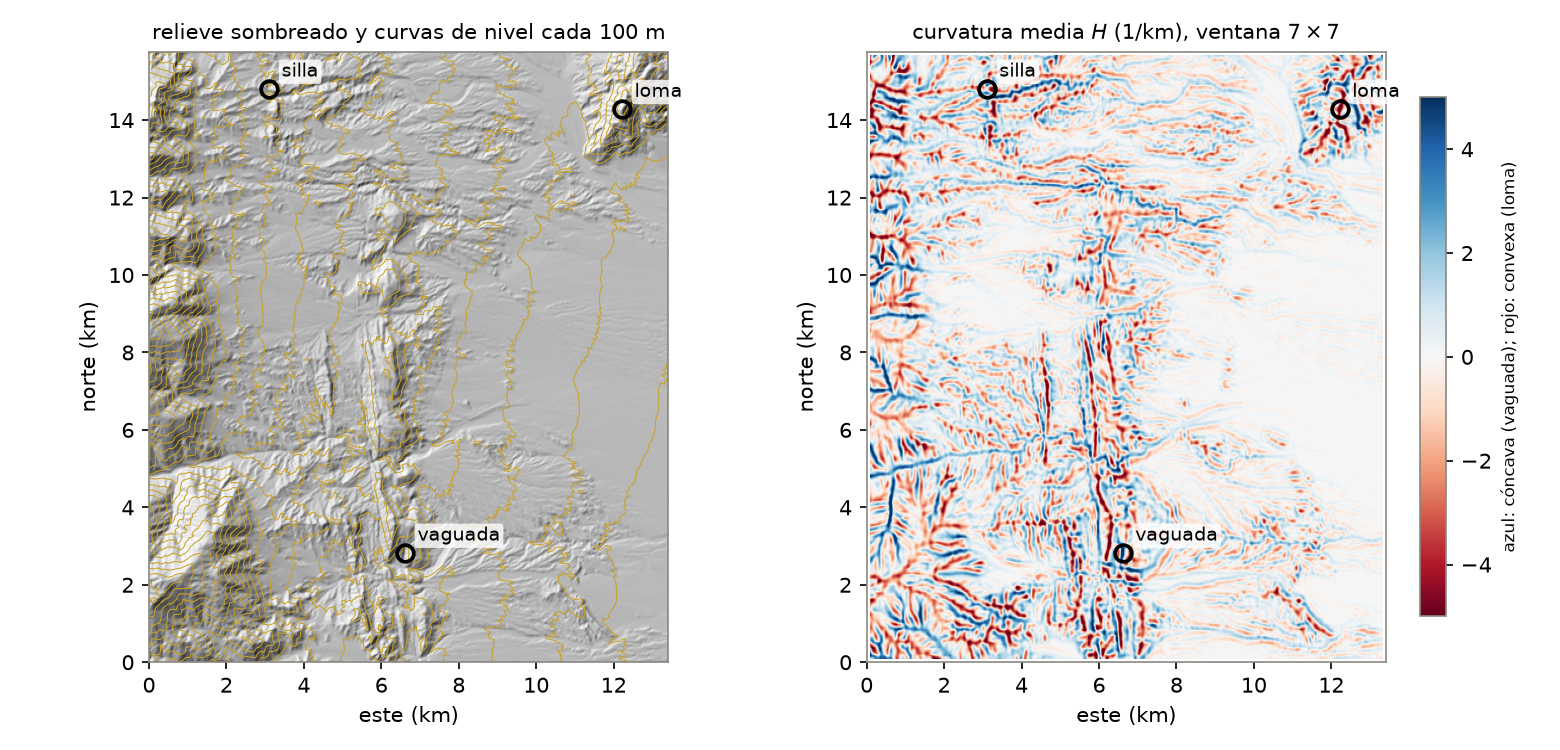
\includegraphics[width=\linewidth]{figuras/curvatura/curv_dem.png}
\caption{Recorte de \(512\times512\) celdas del DEM Copernicus GLO-30 en la precordillera de
Mendoza, en km desde la esquina suroeste. Izquierda: relieve sombreado con curvas de nivel cada
\(100\) m y los tres puntos del cuadro~\ref{tab:curv-dem}. Derecha: curvatura media \(H\) de
la cuadrática ajustada en ventanas de \(7\times7\) celdas, recortada a \(\pm5\) 1/km; en
azul las zonas cóncavas (vaguadas), en rojo las convexas (filos y lomas). Datos: Copernicus DEM GLO-30, \enquote{\textcopyright{} DLR e.V. 2010-2014 and \textcopyright{} Airbus Defence and Space GmbH 2014-2018 provided under COPERNICUS by the European Union and ESA}.}
\label{fig:curv-dem}
\end{figure}

\unidadInteractiva{12_curvatura}{Curvatura como forma cuadrática}{Explorá: con «loma: terreno suave» mové el punto por la superficie y mirá cómo las direcciones principales (teal y óxido) dejan de seguir la grilla \((x,y)\) y \(F\), \(M\) dejan de ser cero, como en los puntos del DEM. Buscá un punto donde \(K\) cambie de signo: ahí pasás de una zona de loma o vaguada a una de silla.}

\section{Ejercicios con solución}

\begin{ejercicio}\label{ex:curv-cuadratica}
Para \(z=x^2+xy+y^2\) en el origen, hallá \(I\), \(II\), las curvaturas y direcciones
principales, \(K\) y \(H\), y verificá la fórmula de Euler en el rumbo del eje \(x\).
\end{ejercicio}
\solucion{El gradiente se anula, \(I\) es la identidad e \(II\) es la hessiana
\(\left(\begin{smallmatrix}2&1\\1&2\end{smallmatrix}\right)\). Sus autovalores son
\(\kappa_1=3\), en la dirección \((1,1)/\sqrt2\), y \(\kappa_2=1\), en \((1,-1)/\sqrt2\):
\(K=3\), \(H=2\), punto elíptico. El eje \(x\) forma \(45^\circ\) con \(d_1\), y Euler da
\(3\cos^245^\circ+1\cdot\sin^245^\circ=2\), que es \(h_{xx}=L\).}

\begin{ejercicio}\label{ex:curv-xy}
Clasificá el origen de \(z=xy\): curvaturas y direcciones principales, \(K\), \(H\) y rumbos
asintóticos. ¿Qué curvas de la superficie pasan por el origen en esos rumbos?
\end{ejercicio}
\solucion{\(II=\left(\begin{smallmatrix}0&1\\1&0\end{smallmatrix}\right)\) con \(I\) la
identidad: \(\kappa_1=1\) en \((1,1)/\sqrt2\) y \(\kappa_2=-1\) en \((1,-1)/\sqrt2\); \(K=-1\),
\(H=0\), punto hiperbólico. Los rumbos asintóticos cumplen \(\tan^2\theta=1\), a \(45^\circ\) de
las direcciones principales: son los ejes \(x\) e \(y\). Sobre ellos la superficie contiene a
las rectas \(z=0\), \(y=0\) y \(z=0\), \(x=0\), cuya curvatura es nula. Es la silla del
ejemplo~\ref{ej:curv-silla} girada \(45^\circ\) y escalada.}

\begin{ejercicio}\label{ex:curv-helice}
La hélice \(\gamma(t)=(3\cos t,\ 3\sin t,\ 4t)\) está sobre el cilindro de radio \(3\).
Calculá su curvatura con la fórmula de Euler y el teorema de Meusnier, sin derivar la
hélice, y comprobala con \(\kappa=\lVert\gamma'\times\gamma''\rVert/\lVert\gamma'\rVert^3\).
\end{ejercicio}
\solucion{\(\gamma'=(-3\sin t,\ 3\cos t,\ 4)\) forma con la generatriz \((0,0,1)\) un ángulo
fijo; con la circunferencia horizontal, el ángulo \(\theta\) cumple
\(\cos^2\theta=9/25=0{,}36\) (\(\theta=53{,}13^\circ\)). Con la normal interior el cilindro
tiene \(\kappa_1=1/3\) en la circunferencia y \(\kappa_2=0\) en la generatriz, así que Euler da
\(\kappa_n=\tfrac13\cdot0{,}36=0{,}12\). La aceleración
\(\gamma''=(-3\cos t,\ -3\sin t,\ 0)\) es horizontal y apunta al eje: la normal principal es
la normal de la superficie, \(\varphi=0\), y por Meusnier \(\kappa=\kappa_n=0{,}12=3/25\). Con la
fórmula, \(\gamma'\times\gamma''=(12\sin t,\ -12\cos t,\ 9)\), de norma \(15\), y
\(\lVert\gamma'\rVert=5\): \(\kappa=15/125=0{,}12\), que es \(R/(R^2+c^2)=3/25\) con \(R=3\),
\(c=4\).}

\begin{ejercicio}\label{ex:curv-generalizado}
En un punto de una superficie, con cierta parametrización,
\(I=\left(\begin{smallmatrix}2&1\\1&1\end{smallmatrix}\right)\) e
\(II=\left(\begin{smallmatrix}3&1\\1&1\end{smallmatrix}\right)\). Hallá las curvaturas y
direcciones principales, \(K\) y \(H\). Comprobá que las direcciones son perpendiculares con
la regla \(I\) pero no en el plano de los parámetros, y que los autovalores de \(II\) sola dan
otra cosa.
\end{ejercicio}
\solucion{\(I^{-1}=\left(\begin{smallmatrix}1&-1\\-1&2\end{smallmatrix}\right)\) y
\(S=I^{-1}II=\left(\begin{smallmatrix}2&0\\-1&1\end{smallmatrix}\right)\), triangular:
\(\kappa_1=2\), \(\kappa_2=1\), \(K=2=\det II/\det I=2/1\), \(H=1{,}5\), punto elíptico.
\((S-2I_2)d=0\) da \(d_1=(1,-1)\) y \((S-I_2)d=0\) da \(d_2=(0,1)\). En el plano de los
parámetros \(d_1\cdot d_2=-1\neq0\); con la regla, \(I\,d_2=(1,1)\) y \(d_1^TI\,d_2=1-1=0\).
Los autovalores de \(II\) sola son \(2\pm\sqrt2\approx3{,}414;\ 0{,}586\): no son las
curvaturas, porque ignoran que el paso unitario en los parámetros no mide \(1\) sobre la
superficie.}

\begin{ejercicio}\label{ex:curv-terreno}
En un punto de un terreno donde la pendiente es nula, la cuadrática ajustada a un DEM da
\(d=-4\), \(e=3\) y \(f=1\), en \(10^{-3}\) 1/m (\(x\) hacia el este, \(y\) hacia el norte).
Clasificá el punto e indicá las curvaturas principales en 1/km, sus radios y los acimutes de las
direcciones principales.
\end{ejercicio}
\solucion{Con pendiente nula \(I\) es la identidad e \(II\) es la hessiana
\(\left(\begin{smallmatrix}2d&e\\e&2f\end{smallmatrix}\right)
=\left(\begin{smallmatrix}-8&3\\3&2\end{smallmatrix}\right)\) 1/km. Su traza es \(-6\) y su
determinante \(-25\), así que \(\kappa=-3\pm\sqrt{34}\): \(\kappa_1=2{,}831\) y
\(\kappa_2=-8{,}831\) 1/km, con radios de \(353\) m y \(113\) m. \(K=-25\) 1/km\(^2\): es una
silla (un portezuelo). El autovector de \(\kappa_1\) cumple \(3y=(8+\kappa_1)x\), o sea
\(y=3{,}610\,x\), con acimut \(\arctan(1/3{,}610)=15{,}5^\circ\): en ese rumbo el terreno
sube hacia los dos lados. En el perpendicular, acimut \(105{,}5^\circ\), baja hacia los dos
lados, más fuerte.}
